\documentclass{beamer}
\beamertemplatenavigationsymbolsempty
\usecolortheme{beaver}
\setbeamertemplate{blocks}[rounded=true, shadow=true]
\setbeamertemplate{footline}[page number]

\usepackage[utf8]{inputenc}
\usepackage[english,russian]{babel}
\usepackage{amssymb,amsfonts,amsmath,mathtext}
\usepackage{algorithm}
\usepackage{algpseudocode}
\makeatletter
\renewcommand{\ALG@name}{Алгоритм}
\makeatother

\DeclareMathOperator*{\argmin}{arg\,min}
\DeclareMathOperator*{\argmax}{arg\,max}

%----------------------------------------------------------------------------------------------------------

\title[\hbox to 56mm{Применение стохастической аппроксимации нулевого порядка с техникой запоминания в алгоритме Франка-Вульфа}]{Применение стохастической аппроксимации нулевого порядка с техникой запоминания в алгоритме Франка-Вульфа}
\author[Богданов А. И.]{Богданов Александр Иванович \\
                        $ $ \\ 
                        Научный руководитель: \\
                        к.ф.-м.н. Безносиков А. Н.}
\institute[]{Московский физико-технический институт \\
             (национальный исследовательский университет) \\
             Физтех-школа прикладной математики и информатики \\
             Кафедра <<Интеллектуальные системы>>}
\date{}

%----------------------------------------------------------------------------------------------------------

\begin{document}

%----------------------------------------------------------------------------------------------------------

\begin{frame}

    \maketitle

\end{frame}

%-----------------------------------------------------------------------------------------------------

\begin{frame}{Цель исследования}

    \textbf{Проблема:} Ставится выпуклая задача оптимизации на ограниченном выпуклом множестве с доступом только к зашумленному нулевому оракулу. \\

    $ $\\

    \textbf{Цель:} Предложить робастый алгоритм аппроксимации градиента, использующий $\mathcal{O}(1)$ вызовов оракула на каждой итерации.\\

    $ $\\

    \textbf{Решение:} Предлагается модификация \texttt{JAGUAR}, которая использует технику запоминания.
    
\end{frame}

%-----------------------------------------------------------------------------------------------------

\begin{frame}{Постановка задачи}

    Рассматривается две оптимизационные задачи:\\

    \begin{itemize}
        \item Нестохастическая
                
            \begin{align*}
                \min_{x \in Q} f(x)
            \end{align*}

            Доступ только к $f_{\delta}(x) := f(x) + \delta(x)$, где $\delta(x)$ -- шум.

            $f(x)$ -- выпуклая на $Q$ функция.

        \item Стохастическая
        
            \begin{align*}
                \min_{x \in Q} f(x) :=  \mathbb{E}_{\xi} \left[ f(x, \xi) \right]
            \end{align*}

                
            Доступ только к $f_{\delta}(x, \xi) := f(x, \xi) + \delta(x, \xi)$, где $\delta(x, \xi)$ - шум.

            $f(x, \xi)$ -- выпуклая на $Q$ функция.

    \end{itemize}

        $Q \subseteq \mathbb{R}^d$ -- произвольное выпуклое ограниченное множество.
   
\end{frame}

%----------------------------------------------------------------------------------------------------------

\begin{frame}{Обычный алгоритм Франка-Вульфа}

    Общие допущения:
    \begin{enumerate}
        \item Ограниченность множества $Q$:
            \begin{align*}
                \forall\ x, y \in Q: \|x - y\|^2 \leq D^2.
            \end{align*}
        \item Выпуклость множества $Q$:
            \begin{align*}
                \forall\ 0 \leq \alpha \leq 1, \forall\ x, y \in Q: \alpha x + (1-\alpha) y \in Q.
            \end{align*}
    \end{enumerate}

    \begin{algorithm}[H]
        \caption{Франк-Вульф}
        \begin{algorithmic}[1]
            \State {\bf Вход:} $x_0 \in Q$, $\gamma_k$
        	\For {k = 0, 1, 2, ... , N}
                \State $s^k = \argmin\limits_{s \in Q} \left\{ \left<s, \nabla f(x^k) \right> \right\}$
                \State $x^{k+1} = x^k + \gamma_k (s^k - x^k)$
            \EndFor
            \State {\bf Выход:} $x^{N + 1}$ 
        \end{algorithmic}
    \end{algorithm}

\end{frame}

%----------------------------------------------------------------------------------------------------------

\begin{frame}{Франк-Вульф с \texttt{JAGUAR} в нестохастическом случае}

    Схема аппроксимации:
    \begin{align*}
        \widetilde{\nabla}_i f_\delta (x) :=  \frac{f_\delta (x + \tau e_i) - f_\delta(x - \tau e_i)}{2 \tau} e_i,
    \end{align*}
    где $e_i$ -- $i$-ый базисный вектор, $\tau$ -- параметр сглаживания.
    
    \begin{algorithm}[H]
        \caption{ФВ с \texttt{JAGUAR} в нестохастическом случае}
        \begin{algorithmic}
            \State {\bf Вход:} $x^0 \in Q$, $h^0 = \widetilde\nabla f_{\delta}(x^0)$, $\gamma_k$, $\tau$
            \For{ $k = 0, 1, 2, ... , N$ }
                \State Сэмплируем $i \in \overline{1, d}$ независимо и равномерно
                \State Считаем $\widetilde{\nabla}_i f_\delta (x^k) = \frac{f_\delta (x^k + \tau e_i) - f_\delta (x^k - \tau e_i)}{2 \tau} e_i$
                \State  $h^{k + 1} = h^k - \langle h^k, e_i \rangle e_i + \widetilde{\nabla}_i f_{\delta}(x^k)$
                \State $s^k = \argmin\limits_{x \in Q} \left<s, h^{k + 1} \right>$
                \State $x^{k + 1} = x^k + \gamma_k (s^k - x^k)$
            \EndFor
            \State {\bf Выход:} $x^{N + 1}$
        \end{algorithmic}
    \end{algorithm}
        
\end{frame}

%----------------------------------------------------------------------------------------------------------

\begin{frame}{Франк-Вульф с \texttt{JAGUAR} в нестохастическом случае}

    Допущения:
    \begin{enumerate}
        \item Функция $f(x)$ $L$-гладкая на множестве $Q$: 
            \begin{align*}
                \forall\ x, y \in Q: \left\| \nabla f(x) - \nabla f(y) \right\| \leq L \left\| x - y\right\|.
            \end{align*}

        \item Функция $f(x)$ выпукла на множестве $Q$:
            \begin{align*}
                \forall\ x, y \in Q: f(y) \geq f(x) + \langle \nabla f(x), y - x \rangle.
            \end{align*}

        \item Ограниченность оракульного шума:
            \begin{align*}
                \exists\ \Delta > 0 \forall\ x \in Q: |\delta(x)|^2 \leq \Delta^2.
            \end{align*}
                
    \end{enumerate}

\end{frame}

%----------------------------------------------------------------------------------------------------------

% \begin{frame}{Франк-Вульф с \texttt{JAGUAR} в нестохастическом случае}

%     \textbf{Теорема (Богданов, 2023)} При шаге оптимизатора:
%     \begin{align*}
%         \gamma_k = \frac{4}{k + 8d}
%     \end{align*}  
%     получается оценка на градиент:
%     \small{
%         \begin{align*}
%             \mathbb{E} \left[\left\|h^{k} - \nabla f(x^{k})\right\|^2 \right] = \mathcal{O}
%             &\Bigg(
%             d L^2 \gamma^2 + \frac{d \Delta^2}{\gamma^2} \\
%             &+
%             \frac{\max \{d^2 L^2 D^2, \|h^0 - \nabla f(x^0)\|^2 \cdot d^2\}}{(k + d)^2}
%             \Bigg).
%         \end{align*}
%     }

%     Если $h_0 = \widetilde{\nabla} f_\delta(x^0)$, то можно упростить:
    
%     \begin{align*}
%         \mathbb{E} \left[\left\|h^{k} - \nabla f(x^{k})\right\|^2 \right] = \mathcal{O} \left( d L^2 \gamma^2 + \frac{d \Delta^2}{\gamma^2} + \frac{d^2 L^2 D^2}{(k + 8d)^2} \right).
%     \end{align*}
        
% \end{frame}

%----------------------------------------------------------------------------------------------------------

\begin{frame}{Франк-Вульф с \texttt{JAGUAR} в нестохастическом случае}

    \textbf{Теорема (Богданов, 2023)} При шаге оптимизатора:
    \begin{align*}
        \gamma_k = \frac{4}{k + 8d}
    \end{align*}  
    получается оценка на сходимость:
    \small{
        \begin{align*}
            \mathbb{E} \left[ f(x^{N}) - f(x^*) \right] = \mathcal{O} \left( \frac{d \max\{L D^2, f(x^0) - f(x^*)\}}{N + 8d} + \sqrt{d} L D \gamma + \frac{\sqrt{d} \Delta D}{\gamma}\right).
            \end{align*}
    }
    \textbf{Следствие} Пусть $\varepsilon$ определяет точность: $\mathbb{E} \left[f(x^N) - f(x^*) \right] \leq \varepsilon$:
    \begin{align*}
        N = \mathcal{O} \left( \frac{d \max\{L D^2, f(x^0) - f(x^*)\}}{\varepsilon} \right),
    \end{align*}
    \begin{align*}
        \gamma = \mathcal{O} \left(\frac{\varepsilon}{\sqrt{d} L D} \right), \quad
        \Delta = \mathcal{O} \left( \frac{\varepsilon^2}{d L D^2}\right).
    \end{align*}

\end{frame}

%----------------------------------------------------------------------------------------------------------

\begin{frame}{Эксперимент для нестохастического случая}

    Эксперимент проводился на симплексном множестве на датасете "mushrooms".

    \begin{figure}
        \centering
        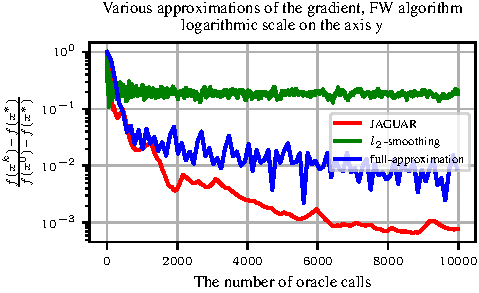
\includegraphics[width = 0.9\textwidth]{BachelorThesis_slides/pictures/Non_stochastics_FW_LogReg_Simplex.pdf}
    \end{figure}

\end{frame}

%----------------------------------------------------------------------------------------------------------

\begin{frame}{Эксперимент для нестохастического случая}

    Эксперимент проводился на симплексном множестве на квадратичной задаче.

    \begin{figure}
        \centering
        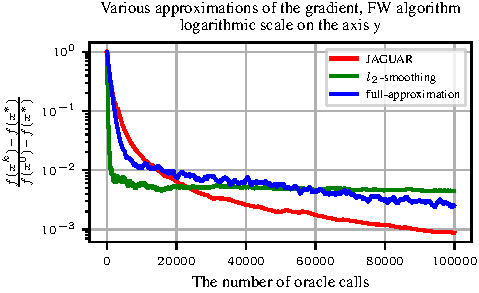
\includegraphics[width = 0.9\textwidth]{BachelorThesis_slides/pictures/Non_stochastics_FW_Reg_Simplex.pdf}
    \end{figure}

\end{frame}

%----------------------------------------------------------------------------------------------------------

\begin{frame}{Франк-Вульф с \texttt{JAGUAR} в стохастическом случае}

    Схемы аппроксимации:
    \begin{itemize}
        \item Двухточечная обратная связь (ДОС):
            \begin{align*}
                \widetilde{\nabla}_i f_\delta (x, \xi) :=  \frac{f_\delta (x + \tau e_i, \xi) - f_\delta (x - \tau e_i, \xi)}{2 \tau} e_i,
            \end{align*}
        \item Одноточечная обратная связь (ООС):
            \begin{align*}
                \widetilde{\nabla}_i f_\delta (x, \xi^+, \xi^-) :=  \frac{f_\delta (x + \tau e_i, \xi^+) - f_\delta (x - \tau e_i, \xi^-)}{2 \tau} e_i,
            \end{align*}
    \end{itemize}
    где $e_i$ -- $i$-ый базисный вектор, $\tau$ -- параметр сглаживания.

\end{frame}

%----------------------------------------------------------------------------------------------------------

\begin{frame}{Франк-Вульф с \texttt{JAGUAR} в стохастическом случае}

    \begin{algorithm}[H]
        \caption{ФВ с \texttt{JAGUAR} в стохастическом случае}
        \begin{algorithmic}
        \State {\bf Вход:} $x^0 \in Q$, $h^0 = g^0 = \widetilde{\nabla} f_\delta (x^0, \xi_{\overline{1, d}}^\pm)$, $\gamma_k$, $\eta_k$, $\tau$
        \For {$k = 0, 1, 2, ... , N$}
            \State Сэмплируем $i \in \overline{1, d}$ независимо и равномерно
            \State Сэмплируем 2 реализации $\xi$: $\xi^+_k$ и $\xi^-_k$ независимо (в ДОС $\xi_k^+= \xi_k^-$)
            \State Считаем $\widetilde{\nabla}_{i_k} f_\delta (x^k, \xi^+_k, \xi^-_k) = \frac{f_\delta (x^k + \tau e_{i_k}, \xi^+_k) - f_\delta (x^k - \tau e_{i_k}, \xi^-_k)}{2 \tau} e_{i_k}$
            \State $h^{k+1} = h^k - \langle h^k, e_{i_k} \rangle e_{i_k} + \widetilde{\nabla}_{i_k} f_\delta (x^k, \xi^+_k, \xi^-_k)$
            \State $\rho^{k} = h^{k} - d \cdot \langle h^{k}, e_{i_k} \rangle e_{i_k} + d \cdot \widetilde{\nabla}_{i_k} f_\delta (x^k, \xi^+_k, \xi^-_k)$
            \State $g^{k + 1} = (1 - \eta_k) g^k + \eta_k \rho^k$
            \State $s^k = \argmin\limits_{s \in Q} \left<s, g^{k+1} \right>$
            \State $x^{k + 1} = x^k + \gamma_k (s^k - x^k)$
        \EndFor
        \State \textbf{Выход:} $x^{N + 1}$
        \end{algorithmic}
   \end{algorithm}
  
\end{frame}

%----------------------------------------------------------------------------------------------------------

\begin{frame}{Франк-Вульф с \texttt{JAGUAR} в стохастическом случае}

    Допущения:
    \small{
        \begin{enumerate}
            \item Функция $f(x, \xi)$ $L(\xi)$-гладкая на множестве $Q$: 
                \begin{align*}
                    \forall\ x, y \in Q: \left\| \nabla f(x, \xi) - \nabla f(y, \xi) \right\| \leq L(\xi) \left\|x-y\right\|.
                \end{align*}
            \item Функция $f(x, \xi)$ выпукла на множестве $Q$:
                \begin{align*}
                    \forall\ x, y \in Q: f(y, \xi) \geq f(x, \xi) + \langle \nabla f(x, \xi), y - x \rangle.
                \end{align*}
            \item Ограниченность оракульного шума:
                \begin{align*}
                    \exists\ \Delta > 0: \forall\ x \in Q: \mathbb{E} \left[ |\delta(x, \xi)|^2 \right] \leq \Delta^2
                \end{align*}
            \item Ограниченность второго момента градиента:
                \begin{align*}
                    \exists\ \sigma^2_{\nabla}: \mathbb{E} \left[ \| \nabla f(x, \xi) - \nabla f(x) \|^2 \right] \leq \sigma^2_{\nabla}
                \end{align*}
            \item Ограниченность второго момента оракула (для ООС):
                \begin{align*}
                    \exists\ \sigma^2_{f}: \mathbb{E} \left[ \left|f(x, \xi) - f(x) \right|^2 \right] \leq \sigma^2_{f}
                \end{align*}
        \end{enumerate}
    }

\end{frame}

%----------------------------------------------------------------------------------------------------------

% \begin{frame}{Франк-Вульф с \texttt{JAGUAR} в стохастическом случае}

%     \textbf{Теорема (Богданов, 2023)} При шаге оптимизатора и шаге моментума:
%     \begin{align*}
%         \gamma_k = \frac{4}{k + 8d^{3/2}}, \quad \eta_k = \frac{4}{(k + 8d^{3/2})^{2/3}}
%     \end{align*}  
%     получается оценка на градиент:
%     \small{
%         \begin{align*}
%             \mathbb{E} \left[ \| g^k - \nabla f(x^k) \|^2 \right]
%             &=
%             \mathcal{O} \Bigg( \frac{d^4 \|h^0 - \nabla f(x^0)\|^2}{(k + 8d^{3/2})^{8/3}} + d L^2 \gamma^2 + \frac{d \Delta^2}{\gamma^2}
%             \\&+
%             \frac{L^2 D^2 + \max\{d^2 \sigma_f^2/ \gamma^2 + d^2 \sigma_{\nabla}^2, d \|g^0 - \nabla f(x^0)\|^2\}}{(k + 8d^{3/2})^{2/3}} \Bigg)
%         \end{align*}
%     }
%     Если $h^0 = g^0 = \widetilde{\nabla} f_\delta (x^0, \xi^+_1, \xi^-_1, ..., \xi^+_d, \xi^-_d)$, то можно упростить:
%     \begin{align*}
%         \mathbb{E} \left[ \| g^k - \nabla f(x^k) \|^2 \right] = \mathcal{O} \left(\frac{L^2 D^2 + d^2 \sigma_f^2/ \gamma^2 + d^2 \sigma_{\nabla}^2}{(k + 8d^{3/2})^{2/3}} + d L^2 \gamma^2 + \frac{d \Delta^2}{\gamma^2} \right)
%     \end{align*}
            
% \end{frame}

%----------------------------------------------------------------------------------------------------------

\begin{frame}{Франк-Вульф с \texttt{JAGUAR} в стохастическом случае}

    \textbf{Теорема (Богданов, 2023)} При шаге оптимизатора и шаге моментума:
    \begin{align*}
        \gamma_k = \frac{4}{k + 8d^{3/2}}, \quad \eta_k = \frac{4}{(k + 8d^{3/2})^{2/3}}
    \end{align*}
    получается оценка на сходимость:
    \small{
        \begin{align*}
            \mathbb{E}\left[f(x^{N}) - f(x^*) \right] = \mathcal{O}
            &\Bigg(
            \frac{L D^2 + d \sigma_f D/ \gamma + d \sigma_{\nabla} D + \sqrt{d} (f(x^0) - f(x^*))}{(N + 8d^{3/2})^{1/3}} \\
            &+
            \sqrt{d} L D \gamma + \frac{\sqrt{d} \Delta D}{\gamma} \Bigg)
        \end{align*}
    }
    \textbf{Следствие} Пусть $\varepsilon$ определяет точность: $\mathbb{E} \left[ f(x^N) - f(x^*) \right] \leq \varepsilon$:
    \begin{align*}
        N = \mathcal{O} \left( \max\left\{ \left[ \frac{L D^2 + d\sigma_{\nabla} D + \sqrt{d} (f(x^0) - f(x^*))}{\varepsilon}\right]^3 , \frac{d^{9/2} \sigma_f^3 L^3D^6}{\varepsilon^6} \right\}\right),
    \end{align*}
    \begin{align*}
        \gamma = \mathcal{O} \left(\frac{\varepsilon}{\sqrt{d} L D} \right), \quad \Delta = \mathcal{O} \left( \frac{\varepsilon^2}{d L D^2}\right).
    \end{align*}
            
\end{frame}

%----------------------------------------------------------------------------------------------------------

\begin{frame}{Эксперимент}

    Эксперимент проводился на $L2$-шаре на квадратичной задаче.

    \begin{figure}
        \centering
        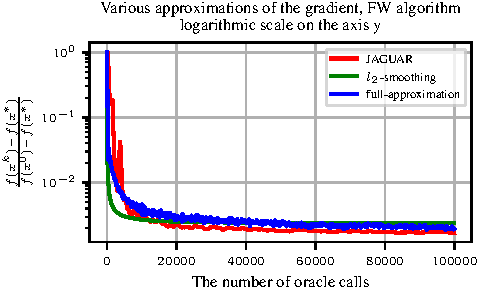
\includegraphics[width = 0.9\textwidth]{BachelorThesis_slides/pictures/Stochastics_TPF_FW_Reg_L2.pdf}
    \end{figure}

\end{frame}

%----------------------------------------------------------------------------------------------------------

\begin{frame}{Эксперимент}

    Эксперимент проводился на симплексном множестве на квадратичной задаче.

    \begin{figure}
        \centering
        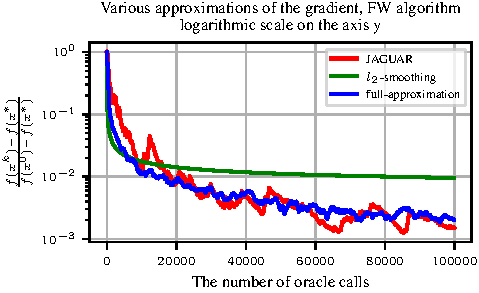
\includegraphics[width = 0.9\textwidth]{BachelorThesis_slides/pictures/Stochastics_TPF_FW_Reg_Simplex.pdf}
    \end{figure}

\end{frame}

%----------------------------------------------------------------------------------------------------------

\begin{frame}{Выносится на защиту}

    \begin{enumerate}
        \item Для выпуклой задачи оптимизации на ограниченном выпуклом множестве с доступом только к зашумленному нулевому оракулу предложен и исследован метод \texttt{JAGUAR} для алгоритма Франка-Вульфа.
        \item Доказаны теоретические оценки сходимости использования данного метода для нестохастического и стохастического случаев в алгоритме Франка-Вульфа. Показано теоретическое превосходство над $l_2$-сглаживанием и полной аппроксимаций. 
        \item Проведены вычислительные эксперименты, в которых сравнивается \texttt{JAGUAR}-аппроксимация с $l_2$-сглаживанием и полной аппроксимаций на различных задачах минимизации. Показано практическое превосходство.
    \end{enumerate}

\end{frame}

%-----------------------------------------------------------------------------------------------------

\begin{frame}{Литература}
    \begin{itemize}
        \item Marguerite Frank and Philip Wolfe. An algorithm for quadratic programming. Naval research logistics quarterly, 3(1-2):95–110, 1956.
        \item Darina Dvinskikh, Vladislav Tominin, Iaroslav Tominin, and Alexander Gasnikov. Noisy zeroth-order optimization for non-smooth saddle point problems. In International Conference on Mathematical Optimization Theory and Operations Research, pages 18–33. Springer, 2022.
        \item Anit Kumar Sahu, Manzil Zaheer, and Soummya Kar. Towards gradient free and projection free stochastic optimization. In The 22nd International Conference on Artificial Intelligence and Statistics, pages 3468–3477. PMLR, 2019.
    \end{itemize}

\end{frame}

%----------------------------------------------------------------------------------------------------------

\end{document}